\documentclass[tikz,border=5pt]{standalone}
\usepackage{tikz}
\usetikzlibrary{shapes.geometric,arrows.meta,positioning,calc,backgrounds}

\newcommand{\shapetext}[1]{{\tiny\color{gray!70!black}#1}}

\begin{document}
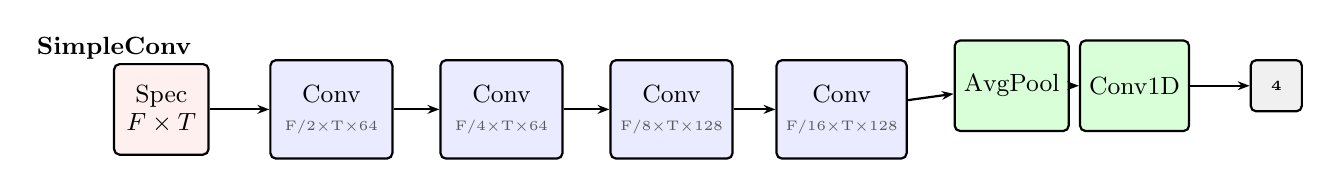
\begin{tikzpicture}[
  x=1.2cm, y=1.2cm,
  font=\small,
  encblock/.style={rectangle, draw, thick, fill=blue!8, rounded corners=2pt, minimum width=1.55cm, minimum height=1.25cm, align=center},
  headblock/.style={rectangle, draw, thick, fill=green!15, rounded corners=2pt, minimum width=1.3cm, minimum height=1.15cm, align=center},
  inputblock/.style={rectangle, draw, thick, fill=red!6, rounded corners=2pt, minimum width=1.2cm, minimum height=1.15cm, align=center},
  outblock/.style={rectangle, draw, thick, fill=gray!12, rounded corners=2pt, minimum width=0.65cm, minimum height=0.65cm, align=center, font=\bfseries\tiny},
  arrow/.style={-{Stealth[length=1.5mm]}, thick},
  label/.style={font=\bfseries\small},
]

\node[label] at (-7.3,0.65) {SimpleConv};
\node[inputblock] (a-in) at (-6.8,0) {Spec\\[-1pt]$F\times T$};
\node[encblock] (a-b1) at (-5.0,0) {Conv\\[-1pt]\shapetext{F/2$\times$T$\times$64}};
\node[encblock] (a-b2) at (-3.2,0) {Conv\\[-1pt]\shapetext{F/4$\times$T$\times$64}};
\node[encblock] (a-b3) at (-1.4,0) {Conv\\[-1pt]\shapetext{F/8$\times$T$\times$128}};
\node[encblock] (a-b4) at (0.4,0) {Conv\\[-1pt]\shapetext{F/16$\times$T$\times$128}};
\node[headblock] (a-h1) at (2.2,0.25) {AvgPool};
\node[headblock] (a-h2) at (3.5,0.25) {Conv1D};
\node[outblock] (a-out) at (5.0,0.25) {4};
\draw[arrow] (a-in) -- (a-b1);
\draw[arrow] (a-b1) -- (a-b2);
\draw[arrow] (a-b2) -- (a-b3);
\draw[arrow] (a-b3) -- (a-b4);
\draw[arrow] (a-b4) -- (a-h1);
\draw[arrow] (a-h1) -- (a-h2);
\draw[arrow] (a-h2) -- (a-out);

\end{tikzpicture}
\end{document}
